\chapter{Imunitas Adaptif dan Vaksinasi}\label{ch:b3:adaptive-immunity}

Pada tahun 1796 seorang dokter desa menggores nanah dari luka cacar sapi
seorang pemerah susu ke lengan seorang anak lelaki, lalu enam minggu kemudian
menginokulasinya dengan cacar; anak itu tidak jatuh sakit. Pada tahun 1980
Organisasi Kesehatan Dunia menyatakan cacar --- yang telah membunuh tiga ratus
juta orang pada abad kedua puluh --- terbasmi dari Bumi, dengan cara itu.
Sistem yang direkrut Jenner, tanpa tahu bahwa sistem itu ada, dapat
mengenali molekul apa pun yang tidak pernah dijumpainya, memilih dari seratus
miliar reseptor yang berbeda beberapa yang cocok, melipatgandakan sel yang
mengusungnya sejuta kali lipat dalam sepekan, memperbaiki kecocokannya lewat
mutasi dan seleksi sambil melakukannya, lalu mengingat hasilnya seumur hidup; ia
juga belajar untuk tidak menyerang tubuh yang membuatnya, dan kegagalannya
mempelajari itu adalah penyakit autoimun. Bab ini memperlakukan
\omterm{def:b3:adaptive-immunity:lymphocytes}{limfosit} dan bagaimana mereka membuat reseptornya, bagaimana sebuah tanggapan
ditegakkan dan diingat, bagaimana \omterm{def:b3:adaptive-immunity:tolerance}{toleransi} ditegakkan dan hilang, serta
aritmetika yang dengannya memvaksinasi cukup banyak orang melindungi mereka yang
tidak divaksinasi.

\section{Limfosit dan seleksi klonal}

\begin{definition}[Limfosit dan reseptornya]\label{def:b3:adaptive-immunity:lymphocytes}
\index{limfosit}\index{sel B}\index{sel T}%
\index{antigen}\index{seleksi klonal}\index{kelenjar limfa}
\emph{Imunitas adaptif} diusung \emph{limfosit}: \emph{sel~B},
yang matang di dalam sumsum tulang dan reseptor antigennya sebuah
\emph{\omterm{def:b3:adaptive-immunity:antibody}{antibodi}} terikat selaput yang kemudian disekresikannya; serta \emph{sel~T},
yang matang di dalam \omterm{def:b3:adaptive-immunity:tolerance}{timus} dan reseptornya mengenali
serpihan peptida yang dipajang pada permukaan sel lain. Sebuah
\emph{antigen} adalah apa pun yang diikat sebuah reseptor; bagian yang
benar-benar disentuh adalah sebuah \emph{epitop}. Fakta pendirinya adalah
\emph{seleksi klonal} (Burnet, 1957): tiap limfosit mengusung reseptor satu
kekhasan saja, yang terpancang sebelum ia menjumpai antigen apa pun; tubuhnya
memuat sebuah khazanah berisi sekitar $10^{11}$ sel semacam itu; sebuah antigen
memilih beberapa yang reseptornya cocok lalu mendorongnya membelah menjadi
sebuah klona sel efektor dan \omterm{def:b3:adaptive-immunity:response}{sel ingatan}; dan limfosit yang reseptornya cocok
dengan molekul tubuhnya sendiri dihapus atau dibungkam sewaktu matang. Selnya
beredar terus-menerus antara darah dan \emph{kelenjar limfa},
limpa, serta jaringan limfoid mukosa, tempat antigen yang diusung \omterm{def:b3:innate-immunity:innate}{sel dendritik}
(\cref{ch:b3:innate-immunity}) dipajang, sehingga sel yang cocok dan
langka --- satu dari seratus ribu bagi sebuah epitop tertentu ---
menemukannya dalam sehari atau dua hari.
\end{definition}

\begin{proof}[Bukti eksperimental]
Nossal dan Lederberg (1958) menaruh \omterm{def:b3:adaptive-immunity:lymphocytes}{limfosit} tunggal dari tikus yang
diimunisasi ke dalam tetesan mikro lalu menguji \omterm{def:b3:adaptive-immunity:antibody}{antibodi} yang disekresikan
masing-masing: tiap sel membuat \omterm{def:b3:adaptive-immunity:antibody}{antibodi} terhadap satu dari kedua \omterm{def:b3:adaptive-immunity:lymphocytes}{antigennya},
tidak pernah keduanya. Burnet telah meramalkannya setahun sebelumnya. Tonegawa
(1976) membandingkan DNA sebuah gen \omterm{def:b3:adaptive-immunity:antibody}{antibodi} pada sel embrio dan pada sebuah
\omterm{def:b3:cancer-biology:hallmarks}{tumor} penyekresi \omterm{def:b3:adaptive-immunity:antibody}{antibodi}: pada embrionya bagian berubah-ubah dan bagian
tetapnya terletak berjauhan, pada \omterm{def:b3:cancer-biology:hallmarks}{tumornya} keduanya tersambung --- gennya telah
dipotong dan disambung di dalam sel somatiknya, yakni pembuktian pertama sebuah
genom yang disusun ulang dengan sengaja.
\end{proof}

\section{Membuat seratus miliar reseptor}

\begin{definition}[Struktur antibodi dan rekombinasi V(D)J]\label{def:b3:adaptive-immunity:antibody}
\index{antibodi}\index{imunoglobulin}\index{rekombinasi V(D)J}%
\index{RAG}\index{keanekaan sambungan}\index{penukaran kelas}
Sebuah \emph{antibodi} (imunoglobulin) adalah dua rantai berat yang serupa dan
dua rantai ringan yang serupa, masing-masing dengan sebuah \omterm{def:b3:structural-biology:levels}{domain}
\emph{berubah-ubah} di ujungnya dan \omterm{def:b3:structural-biology:levels}{domain} \emph{tetap} di belakangnya; kedua
lengannya masing-masing mengikat sebuah epitop lewat tiga gelung hipervariabel
\omterm{def:b3:structural-biology:levels}{domain} berubah-ubah rantai beratnya dan tiga gelung rantai ringannya, dan
batangnya (Fc) adalah apa yang dikenali fagosit, \omterm{def:b3:innate-immunity:complement}{komplemen}, dan sel mast. Lima
kelasnya berbeda pada daerah tetap rantai beratnya: IgM, yang pertama dibuat,
sebuah pentamer yang mengaktifkan \omterm{def:b3:innate-immunity:complement}{komplemen} dengan baik; IgG, kuda beban darah
dan jaringan, yang menyeberangi plasenta; IgA, sebuah dimer yang disekresikan
melintasi permukaan mukosa ke dalam usus, saluran napas, dan susu; IgE, yang
diikat sel mast, melawan cacing --- dan penyebab alergi; IgD. \omterm{def:b3:structural-biology:levels}{Domain}
berubah-ubahnya tidak disandi begitu saja. Lokus rantai beratnya memuat sekitar
$40$ segmen \emph{V} yang berfungsi, $25$ segmen \emph{D}, dan $6$ segmen
\emph{J}; sebuah sel~B yang sedang berkembang memilih satu dari tiap jenis lalu
menyambungnya lewat \emph{rekombinasi V(D)J}: enzim RAG1 dan RAG2 memotong pada
urutan isyarat rekombinasi yang mengapit segmennya, dan ujungnya disambung mesin
\omterm{def:b3:dna-repair:dsb}{penyambungan ujung tak homolog} \cref{ch:b3:dna-repair}, dengan nukleotida
dipangkas dan ditambahkan secara acak (oleh enzim TdT) pada tiap sambungan ---
itulah \emph{keanekaan sambungan}, yang jatuh tepat pada gelung hipervariabel
ketiga. Rantai ringannya melakukan hal yang sama dengan V dan J. Sesudah
tanggapannya mulai, \omterm{def:b3:structural-biology:levels}{domain} berubah-ubah yang sama disambungkan ke sebuah daerah
tetap yang lain lewat penyusunan ulang yang kedua, yakni \emph{penukaran kelas},
yang mengubah fungsi antibodinya tetapi bukan kekhasannya.
\end{definition}

\begin{theorem}[Besar khazanahnya]\label{thm:b3:adaptive-immunity:repertoire}
\index{khazanah!kombinatoris}
Dengan $V_{H} = 40$, $D = 25$, $J_{H} = 6$ segmen berat, dan rantai ringan
dari dua lokus dengan $(V_{\kappa}, J_{\kappa}) = (40, 5)$ dan
$(V_{\lambda}, J_{\lambda}) = (30, 4)$, cacah gabungan
berat--ringan yang berbeda yang diperoleh dari pemilihan segmen saja adalah
\[
(40\times 25\times 6)\times(40\times 5 + 30\times 4) = 6000\times 320
= 1.9\times 10^{6}.
\]
\omterm{def:b3:adaptive-immunity:antibody}{Keanekaan sambungan} pada kedua sambungan berat dan satu sambungan ringan
mengalikannya dengan sebuah faktor berorde $10^{4}$--$10^{5}$, yang memberi
sebuah khazanah berpotensi di atas $10^{10}$ dari kurang daripada $200$ segmen
gen --- lebih banyak daripada cacah sel~B di dalam sebuah tubuh, sehingga
khazanah yang sebenarnya adalah sebuah contoh dari yang mungkin. \omterm{def:b3:adaptive-immunity:germinal-centre}{Hipermutasi
somatik} selama tanggapannya (di bawah) lalu menghasilkan ragam dari
tiap reseptor yang terpilih.
\end{theorem}
\begin{proof}
Tiap rantai berat adalah satu V, satu D, dan satu J; tiap rantai ringan satu V
dan satu J dari salah satu lokusnya; rantai berat mana pun berpasangan dengan
rantai ringan mana pun, sehingga cacahnya saling dikalikan (asas perkalian), dan
kedua lokus ringannya dijumlahkan. Faktor sambungannya adalah cacah urutan
berbeda yang dapat dihasilkan pemangkasan dan penambahan acak pada sebuah
sambungan --- setidaknya beberapa lusin tiap sambungan --- yang dipangkatkan
dengan cacah sambungannya; nilai tepatnya tidak terdefinisi, tetapi tiga
sambungan yang masing-masing berhasil $30$--$50$ memberi
$3\times 10^{4}$ sampai $10^{5}$. Cacah bagi reseptor sel~T, dengan dua
rantai yang disusun ulang dengan cara yang sama dan sumbangan sambungan yang
lebih besar, seorde dengan itu.
\end{proof}

\begin{omfigure}
\begin{tikzpicture}[every node/.style={font=\scriptsize}, >=stealth]
  % antibody Y
  \begin{scope}[xshift=0cm]
    % heavy chains
    \draw[very thick, omDef] (0,0) -- (0,1.6) -- (-1.3,3.0); \draw[very thick, omDef] (0.35,0) -- (0.35,1.6) -- (1.65,3.0);
    % light chains
    \draw[very thick, omProp] (-0.45,1.55) -- (-1.75,2.95); \draw[very thick, omProp] (0.8,1.55) -- (2.1,2.95);
    \fill[omThm] (-1.55,3.0) circle (0.12); \fill[omThm] (1.9,3.0) circle (0.12);
    \node[above, align=center] at (-1.5,3.15) {domain berubah-ubah:\\tapak pengikat antigen}; 
    \node[right, align=left] at (0.55,0.5) {batang Fc (tetap):\\kelasnya memutuskan fungsinya};
    \node[left, omProp] at (-0.7,2.1) {ringan}; \node[right, omDef] at (0.4,1.3) {berat};
    \draw[omDef] (0.05,1.1) -- (0.3,1.1); \draw[omDef] (0.05,0.7) -- (0.3,0.7);
  \end{scope}
  % V(D)J locus
  \begin{scope}[xshift=4.2cm, yshift=2.4cm, xscale=0.86]
    \draw[very thick, gray] (0,0) -- (8.2,0);
    \foreach \x in {0.2,0.6,1.0,1.4} \draw[thick, fill=omDef!40] (\x,-0.15) rectangle (\x+0.3,0.15);
    \node[above] at (0.95,0.2) {segmen V ($\sim 40$)}; \node[font=\tiny] at (1.95,0) {$\cdots$};
    \foreach \x in {2.5,2.8,3.1} \draw[thick, fill=omProp!50] (\x,-0.15) rectangle (\x+0.2,0.15);
    \node[above] at (2.9,0.2) {D ($25$)};
    \foreach \x in {3.8,4.1,4.4} \draw[thick, fill=omMeth!50] (\x,-0.15) rectangle (\x+0.2,0.15);
    \node[above] at (4.2,0.2) {J ($6$)};
    \foreach \x/\lab in {5.3/\mu,6.0/\delta,6.7/\gamma,7.4/\alpha} { \draw[thick, fill=gray!30] (\x,-0.15) rectangle (\x+0.5,0.15); \node[above] at (\x+0.25,0.2) {C$_{\lab}$}; }
    \draw[->, thick] (4.1,-0.4) -- (4.1,-1.1) node[midway, right, align=left, font=\tiny] {RAG memotong pada urutan isyaratnya;\\satu V, satu D, satu J disambung,\\TdT menambahkan nukleotida acak};
    % rearranged
    \draw[very thick, gray] (0,-1.5) -- (3.3,-1.5);
    \draw[thick, fill=omDef!40] (1.0,-1.65) rectangle (1.3,-1.35); \fill[omThm] (1.3,-1.65) rectangle (1.4,-1.35);
    \draw[thick, fill=omProp!50] (1.4,-1.65) rectangle (1.6,-1.35); \fill[omThm] (1.6,-1.65) rectangle (1.7,-1.35);
    \draw[thick, fill=omMeth!50] (1.7,-1.65) rectangle (1.9,-1.35);
    \draw[thick, fill=gray!30] (2.6,-1.65) rectangle (3.1,-1.35); \node[above] at (2.85,-1.3) {C$_{\mu}$};
    \node[below, align=center] at (1.45,-1.7) {VDJ tersambung: domain berubah-ubahnya,\\merah: nukleotida sambungan};
    \node[right, align=left, font=\tiny] at (3.4,-2.0) {disambung ke C$_{\mu}$: sebuah rantai berat IgM;\\penukaran kelas kemudian menyambung VDJ\\yang sama ke C$_{\gamma}$ atau C$_{\alpha}$};
  \end{scope}
\end{tikzpicture}

{\small Kiri: sebuah \omterm{def:b3:adaptive-immunity:antibody}{antibodi} --- dua rantai berat dan dua rantai ringan,
dengan \omterm{def:b3:structural-biology:levels}{domain} berubah-ubah di ujungnya yang membentuk dua tapak pengikat, dan
batang tetapnya dibaca oleh sisa sistem imunnya. Kanan: lokus rantai
beratnya sebelum dan sesudah \omterm{def:b3:adaptive-immunity:antibody}{rekombinasi V(D)J}, yang memungut satu segmen dari
tiap jenis lalu menambahkan nukleotida acak pada sambungannya.}
\end{omfigure}

\begin{definition}[Reseptor sel~T dan MHC]\label{def:b3:adaptive-immunity:mhc}
\index{reseptor sel T}\index{kompleks histokompatibilitas utama}%
\index{penyajian antigen}\index{pembatasan MHC}\index{HLA}
\emph{Reseptor sel~T} adalah sebuah molekul dua rantai yang dibangun dengan
rekombinasi yang sama, tidak pernah disekresikan, dan ia tidak mengikat \omterm{def:b3:adaptive-immunity:lymphocytes}{antigen}
yang bebas di dalam larutan: ia mengenali sebuah peptida pendek yang dipegang di
dalam alur sebuah molekul \emph{kompleks histokompatibilitas utama} (MHC) pada
permukaan sel lain. \emph{MHC kelas~I}, pada tiap sel berinti, memajang
peptida sepanjang delapan sampai sepuluh residu yang dipotong proteasom dari
protein sitosolik selnya sendiri --- sebuah contoh dari apa yang sedang dibuat
selnya, termasuk \omterm{def:b3:virology:virus}{virus} apa pun --- kepada sel~T \emph{CD8}, yang membunuh selnya
bila peptidanya asing. \emph{MHC kelas~II}, pada \omterm{def:b3:innate-immunity:innate}{sel dendritik},
\omterm{def:b3:innate-immunity:innate}{makrofag}, dan sel~B, memajang peptida sepanjang tiga belas sampai dua puluh lima
residu dari protein yang telah diambil dan dicerna selnya di dalam
\omterm{def:b3:membrane-traffic:endocytosis}{endosom}, kepada sel~T \emph{CD4}, yang menanggapinya dengan menolong. Sebuah
sel~T \emph{terbatasi}: ia mengenali peptidanya hanya pada alel MHC yang
padanya ia terpilih. Gen MHC-nya (\emph{HLA} pada manusia) adalah yang paling
polimorfik di dalam genom, dengan ribuan alel yang masing-masing berbeda pada
alurnya, sehingga tiap orang memajang contoh peptida yang berbeda dari tiap
protein dan tidak ada patogen yang dapat lolos dari penyajian pada semua orang
--- dan sehingga sebuah organ cangkokan dari donor yang tidak cocok
dikenali sebagai asing oleh sebagian besar sel~T penerimanya.
\end{definition}

\begin{proof}[Bukti eksperimental]
Zinkernagel dan Doherty (1974) menginfeksi mencit dari dua galur kawin dalam
dengan sebuah \omterm{def:b3:virology:virus}{virus} lalu menguji sel~T sitotoksiknya pada sel sasaran yang
terinfeksi: sel~T itu membunuh sel terinfeksi dari galurnya sendiri tetapi bukan
dari galur yang lain, padahal \omterm{def:b3:virology:virus}{virusnya} sama. Sel~T itu melihat \omterm{def:b3:virology:virus}{virusnya} hanya
bersama sebuah molekul MHC diri --- itulah \emph{\omterm{def:b3:adaptive-immunity:mhc}{pembatasan MHC}} --- yang
kemudian dijelaskan ketika struktur hablur sebuah molekul MHC
(Bjorkman, 1987) menunjukkan sebuah alur berisi sebuah peptida, dan reseptor
sel~T terbukti mengikat keduanya bersama-sama.
\end{proof}

\begin{omfigure}
\begin{tikzpicture}[every node/.style={font=\scriptsize}, >=stealth]
  % class I pathway
  \begin{scope}
    \draw[thick, omDef, fill=omDef!8] (0,0) rectangle (6.2,3.6); \node[anchor=north west] at (0.05,3.55) {sel berinti mana pun};
    \node[draw, rounded corners, fill=omThm!20, font=\tiny, align=center] (v) at (1.4,2.6) {protein virus atau diri\\di dalam sitosol};
    \node[draw, rounded corners, fill=gray!20, font=\tiny, align=center] (p) at (1.4,1.5) {proteasom:\\peptida 8--10};
    \node[draw, rounded corners, fill=omDef!25, font=\tiny, align=center] (er) at (4.6,1.5) {RE: dimuatkan pada\\MHC kelas I};
    \draw[->, thick] (v) -- (p); \draw[->, thick] (p) -- node[midway, above, font=\tiny] {TAP} (er);
    \draw[->, thick] (er) -- (4.6,3.55);
    \draw[thick, fill=omDef!40] (4.4,3.6) rectangle (4.8,4.1); \fill[omThm] (4.6,4.2) circle (0.09);
    \node[above, align=center] at (4.6,4.35) {peptida--MHC I\\dilihat sel T CD8: membunuh};
  \end{scope}
  % class II pathway
  \begin{scope}[xshift=7.2cm]
    \draw[thick, omProp, fill=omProp!8] (0,0) rectangle (6.2,3.6); \node[anchor=north west] at (0.05,3.55) {sel dendritik, makrofag, sel B};
    \node[draw, rounded corners, fill=omThm!20, font=\tiny, align=center] (ex) at (1.4,2.6) {protein yang diambil\\ke dalam endosom};
    \node[draw, rounded corners, fill=gray!20, font=\tiny, align=center] (dig) at (1.4,1.5) {dicerna:\\peptida 13--25};
    \node[draw, rounded corners, fill=omProp!30, font=\tiny, align=center] (m2) at (4.6,1.5) {MHC kelas II\\dimuatkan di sini};
    \draw[->, thick] (ex) -- (dig); \draw[->, thick] (dig) -- (m2);
    \draw[->, thick] (m2) -- (4.6,3.55);
    \draw[thick, fill=omProp!50] (4.4,3.6) rectangle (4.8,4.1); \fill[omThm] (4.6,4.2) circle (0.09);
    \node[above, align=center] at (4.6,4.35) {peptida--MHC II\\dilihat sel T CD4: menolong};
  \end{scope}
\end{tikzpicture}

{\small Kedua jalur penyajiannya. Kelas~I menunjukkan kepada sel~T CD8 apa
yang sedang dibuat sebuah sel di dalam dirinya; kelas~II menunjukkan kepada
sel~T CD4 apa yang telah dimakan sebuah sel penyaji \omterm{def:b3:adaptive-immunity:lymphocytes}{antigen}. Tanggapan
sitotoksik diarahkan pada yang pertama, tanggapan penolong pada yang kedua.}
\end{omfigure}

\section{Tanggapannya}

\begin{definition}[Pengaktifan, pertolongan, dan pembunuhan]\label{def:b3:adaptive-immunity:response}
\index{sel T penolong}\index{sel T sitotoksik}\index{kostimulasi}%
\index{sel T pengatur}\index{sel plasma}\index{sel ingatan}
Sebuah sel~T naif diaktifkan ketika reseptornya mengikat peptida--MHC pada
sebuah \omterm{def:b3:innate-immunity:innate}{sel dendritik} yang juga menyediakan kostimulasi (\cref{ch:b3:innate-immunity});
ia lalu membelah tiap enam sampai delapan jam selama sepekan lalu berdiferensiasi.
Sel~T \emph{penolong CD4} berdiferensiasi, menurut \omterm{def:b3:innate-immunity:inflammation}{sitokin} \omterm{def:b3:innate-immunity:innate}{sel
dendritiknya}, menjadi anak himpunan: Th1, yang mengaktifkan \omterm{def:b3:innate-immunity:innate}{makrofag} untuk
membunuh apa yang telah dimakannya (tuberkulosis); Th2, yang mendorong IgE dan
eosinofil melawan cacing; Th17, yang merekrut \omterm{def:b3:innate-immunity:innate}{neutrofil} melawan
bakteri dan jamur di luar sel; penolong folikel, yang menolong
sel~B; serta sel~T \emph{pengatur}, yang menekan. Sel~T \emph{sitotoksik
CD8} membunuh sel yang memajang peptidanya pada kelas~I, dengan
perforin dan granzim serta dengan ligan Fas, yang memicu \omterm{def:b3:cell-cycle-apoptosis:apoptosis}{apoptosis}
(\cref{ch:b3:cell-cycle-apoptosis}) --- yakni pertahanan melawan \omterm{def:b3:virology:virus}{virus} dan
\omterm{def:b3:cancer-biology:hallmarks}{tumor}. Sebuah sel~B diaktifkan oleh \omterm{def:b3:adaptive-immunity:lymphocytes}{antigen} yang mengikat reseptornya ditambah
pertolongan dari sebuah sel~T penolong folikel yang mengenali peptida
\omterm{def:b3:adaptive-immunity:lymphocytes}{antigen} yang sama pada kelas~II sel~B itu; ia lalu menjadi sebuah \emph{sel
plasma} yang menyekresikan ribuan \omterm{def:b3:adaptive-immunity:antibody}{antibodi} tiap detik, selama berhari-hari
(berumur pendek, di dalam kelenjarnya) atau bertahun-tahun (berumur panjang, di
dalam sumsumnya), atau memasuki sebuah \omterm{def:b3:adaptive-immunity:germinal-centre}{pusat germinal}. Sel \emph{ingatan} B dan
T --- berumur panjang, lebih banyak daripada pendahulu naifnya dan lebih cepat
menanggapi --- adalah sisa tiap tanggapan dan dasar vaksinasi.
\end{definition}

\begin{definition}[Pusat germinal]\label{def:b3:adaptive-immunity:germinal-centre}
\index{pusat germinal}\index{hipermutasi somatik}\index{pematangan afinitas}
Di dalam sebuah \emph{pusat germinal}, yakni sebuah struktur yang terbentuk di
sebuah \omterm{def:b3:adaptive-immunity:lymphocytes}{kelenjar limfa} sekitar sepekan sesudah sebuah tanggapan mulai, sel~B yang
aktif menjalankan sebuah algoritme evolusi. Di dalam zona gelapnya mereka
membelah tiap enam jam dan gen berubah-ubah \omterm{def:b3:adaptive-immunity:antibody}{antibodinya} dimutasikan enzim AID
pada sekitar satu perubahan tiap seribu pasangan basa tiap pembelahan --- itulah
\emph{hipermutasi somatik}, yakni sejuta kali laju genomnya, yang diarahkan pada
satu kilobasa. Di dalam zona terangnya tiap sel menguji reseptor barunya
terhadap \omterm{def:b3:adaptive-immunity:lymphocytes}{antigen} yang dipegang \omterm{def:b3:innate-immunity:innate}{sel dendritik} folikel lalu bersaing memperoleh
pertolongan sel~T: sel yang mengikat lebih baik mengambil lebih banyak \omterm{def:b3:adaptive-immunity:lymphocytes}{antigen},
menyajikan lebih banyak, menerima lebih banyak pertolongan, lalu kembali ke zona
gelapnya untuk membelah lagi; sel yang mengikat lebih buruk, atau yang telah
kehilangan pengikatannya, mati lewat \omterm{def:b3:cell-cycle-apoptosis:apoptosis}{apoptosis}. Sepanjang dua sampai
tiga minggu daur, afinitas \omterm{def:b3:adaptive-immunity:antibody}{antibodi} yang selamat naik seratus sampai
seribu kali lipat --- itulah \emph{pematangan afinitas} --- lalu para pemenangnya
pergi sebagai \omterm{def:b3:adaptive-immunity:response}{sel plasma} dan \omterm{def:b3:adaptive-immunity:response}{sel ingatan}, yang juga telah menukar
kelasnya. Tanggapan kedua lebih cepat, lebih besar, dan terbuat dari \omterm{def:b3:adaptive-immunity:antibody}{antibodi}
yang lebih baik karena ia bermula dari populasi yang terpilih, berkembang, dan
tertukar kelas ini.
\end{definition}

\begin{omfigure}
\begin{tikzpicture}[every node/.style={font=\scriptsize}, >=stealth]
  \draw[thick, omDef, fill=omDef!12] (0,0) ellipse (2.7 and 1.7); \node[above, omDef!70!black] at (0,1.75) {zona gelap};
  \draw[thick, omMeth!70!black, fill=omMeth!12] (6.2,0) ellipse (2.7 and 1.7); \node[above, omMeth!60!black] at (6.2,1.75) {zona terang};
  \node[align=center] at (0,0.3) {sel B membelah tiap \qty{6}{h};\\AID memutasikan gen\\antibodinya: $10^{-3}$ tiap bp tiap pembelahan};
  \node[align=center] at (6.2,0.3) {menguji reseptor barunya\\pada antigen yang dipegang\\sel dendritik folikel;\\bersaing memperoleh pertolongan sel T};
  \draw[->, very thick, omProp] (2.4,0.7) .. controls (3.6,1.4) and (4.2,1.4) .. (3.7,0.7); \node[above, omProp] at (3.1,1.45) {mutan keluar};
  \draw[->, very thick, omMeth!70!black] (3.7,-0.7) .. controls (4.2,-1.4) and (3.6,-1.4) .. (2.4,-0.7); \node[below, omMeth!70!black] at (3.1,-1.45) {pemenang kembali, untuk membelah lagi};
  \draw[->, thick, omThm] (6.6,-1.6) -- (6.6,-2.3); \node[below, omThm, align=center] at (6.6,-2.3) {yang kalah: apoptosis\\(kebanyakan mereka)};
  \draw[->, thick] (8.9,0) -- (9.5,0); \node[right, align=left] at (9.5,0) {sesudah 2--3 minggu:\\sel plasma (berumur\\panjang, di dalam sumsum)\\dan sel B ingatan; afinitas\\naik $100$--$1000\times$,\\tertukar kelas};
\end{tikzpicture}

{\small \omterm{def:b3:adaptive-immunity:germinal-centre}{Pusat germinal} sebagai sebuah mesin evolusi: mutasi di dalam
zona gelapnya, seleksi di dalam zona terangnya, lalu berdaur di antara keduanya
sampai \omterm{def:b3:adaptive-immunity:antibody}{antibodi} yang keluar mengikat jauh lebih baik daripada yang masuk.}
\end{omfigure}

\begin{example}[Kinetika sebuah tanggapan]\label{ex:b3:adaptive-immunity:kinetics}
Sekitar satu sel~B dari $10^{5}$ mengikat sebuah epitop tertentu, sehingga
$10^{11}$ sel~B sebuah tubuh memuat sekitar $10^{6}$ pendahulu, yang dari
antaranya mungkin seratus menjumpai \omterm{def:b3:adaptive-immunity:lymphocytes}{antigennya} di dalam kelenjar penyalirnya.
Dengan membelah tiap delapan jam, seratus sel menjadi
$10^{2}\times 2^{21} \approx 2\times 10^{8}$ dalam sepekan. \omterm{def:b3:adaptive-immunity:antibody}{Antibodi} muncul di
dalam serumnya sesudah empat sampai enam hari, IgM lebih dulu, memuncak pada
sekitar dua minggu lalu menurun dengan paruh hidup tiga minggu bagi IgG ketika
\omterm{def:b3:adaptive-immunity:response}{sel plasma} yang berumur pendek mati, lalu menetap pada aras yang dipertahankan
\omterm{def:b3:adaptive-immunity:response}{sel plasma} sumsum yang berumur panjang selama bertahun-tahun. Pemaparan kedua
bermula dari $10^{4}$--$10^{5}$ \omterm{def:b3:adaptive-immunity:response}{sel ingatan} yang berafinitas tinggi dan sudah
tertukar ke IgG: \omterm{def:b3:adaptive-immunity:antibody}{antibodinya} naik dalam dua hari, sepuluh sampai seratus kali
lebih tinggi, lalu menetralkan patogennya sebelum ia dapat mapan --- dan itulah
yang dibeli sebuah \omterm{def:b3:adaptive-immunity:vaccine}{vaksin}.
\end{example}

\begin{omfigure}
\begin{tikzpicture}
\begin{axis}[
  width=0.7\linewidth, height=5.6cm,
  axis x line=bottom, axis y line=left,
  xmin=0, xmax=70, ymin=1, ymax=10000, ymode=log,
  xlabel={hari}, ylabel={antibodi serum (nisbi)},
  xlabel style={font=\small, at={(axis description cs:0.5,-0.12)}, anchor=north}, ylabel style={font=\small},
  tick label style={font=\small}, xtick={0,10,20,30,40,50,60,70},
  clip=false,
]
\addplot[very thick, omDef, domain=0:40, samples=60] {1 + 100*exp(-((x-14)/5)^2) + 15*(1-exp(-x/10))*exp(-(x-14)/60)*(x>14)};
\addplot[very thick, omThm, domain=40:70, samples=60] {1 + 2500*exp(-((x-48)/5)^2) + 400*(1-exp(-(x-40)/4))*(x>40)};
\draw[->, thick, gray] (axis cs:0,0.6) -- (axis cs:0,1.8); \node[font=\scriptsize, gray, anchor=south west] at (axis cs:0.5,1.3) {pemaparan pertama};
\draw[->, thick, gray] (axis cs:40,0.6) -- (axis cs:40,1.8); \node[font=\scriptsize, gray, anchor=south west] at (axis cs:40.5,1.3) {pemaparan kedua};
\node[font=\scriptsize, omDef, anchor=south west] at (axis cs:2,600) {primer: IgM lalu IgG, puncaknya pada dua minggu};
\node[font=\scriptsize, omThm, anchor=south east] at (axis cs:69,3500) {sekunder: lebih cepat, lebih tinggi, IgG, afinitas lebih tinggi};
\end{axis}
\end{tikzpicture}

{\small Tanggapan \omterm{def:b3:adaptive-immunity:antibody}{antibodi} primer dan sekunder. Pemaparan kedua
bermula dari populasi ingatan yang berkembang, tertukar kelas, dan matang
afinitasnya, lalu menjawab dalam hitungan hari pada aras yang tidak pernah
dicapai tanggapan pertamanya.}
\end{omfigure}

\begin{omfigure}
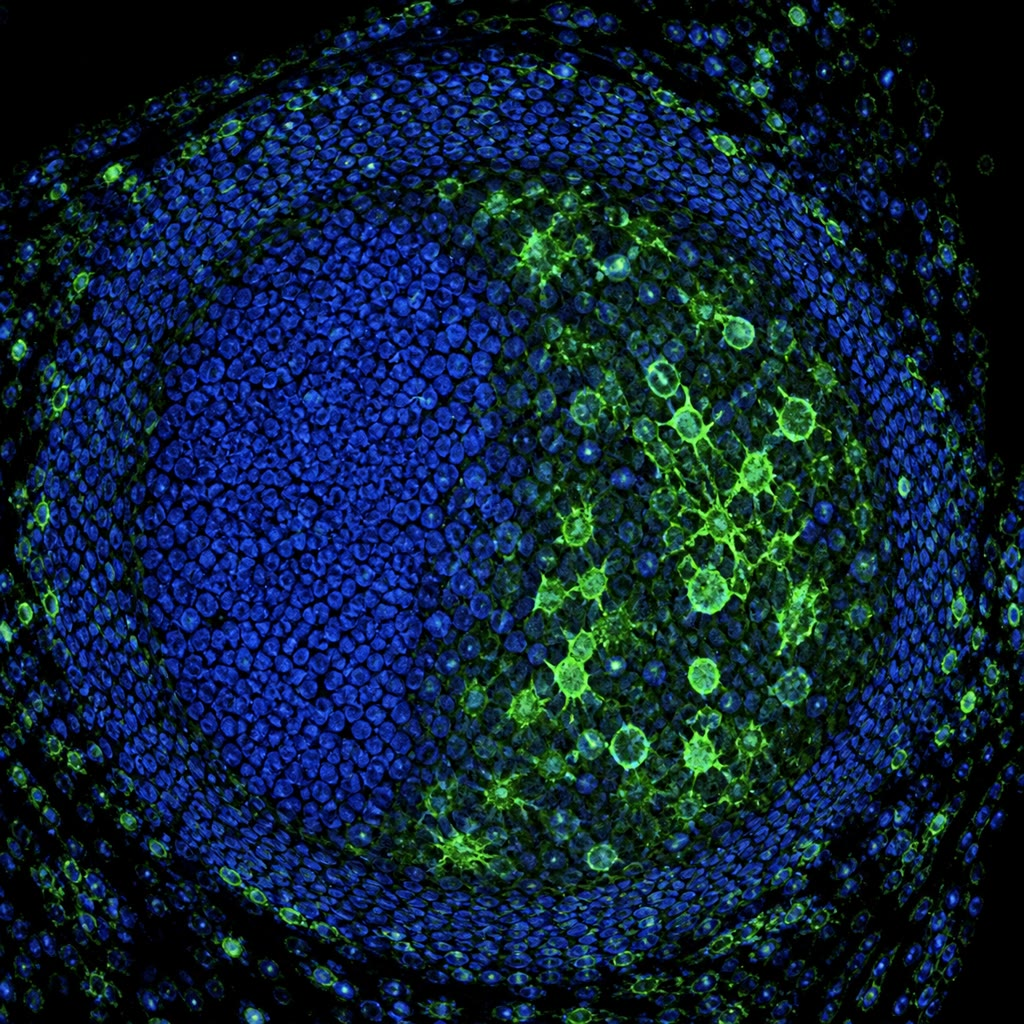
\includegraphics[width=0.36\linewidth]{images/book5/ai/b5-16-germinal-centre.jpg}\hspace{0.04\linewidth}
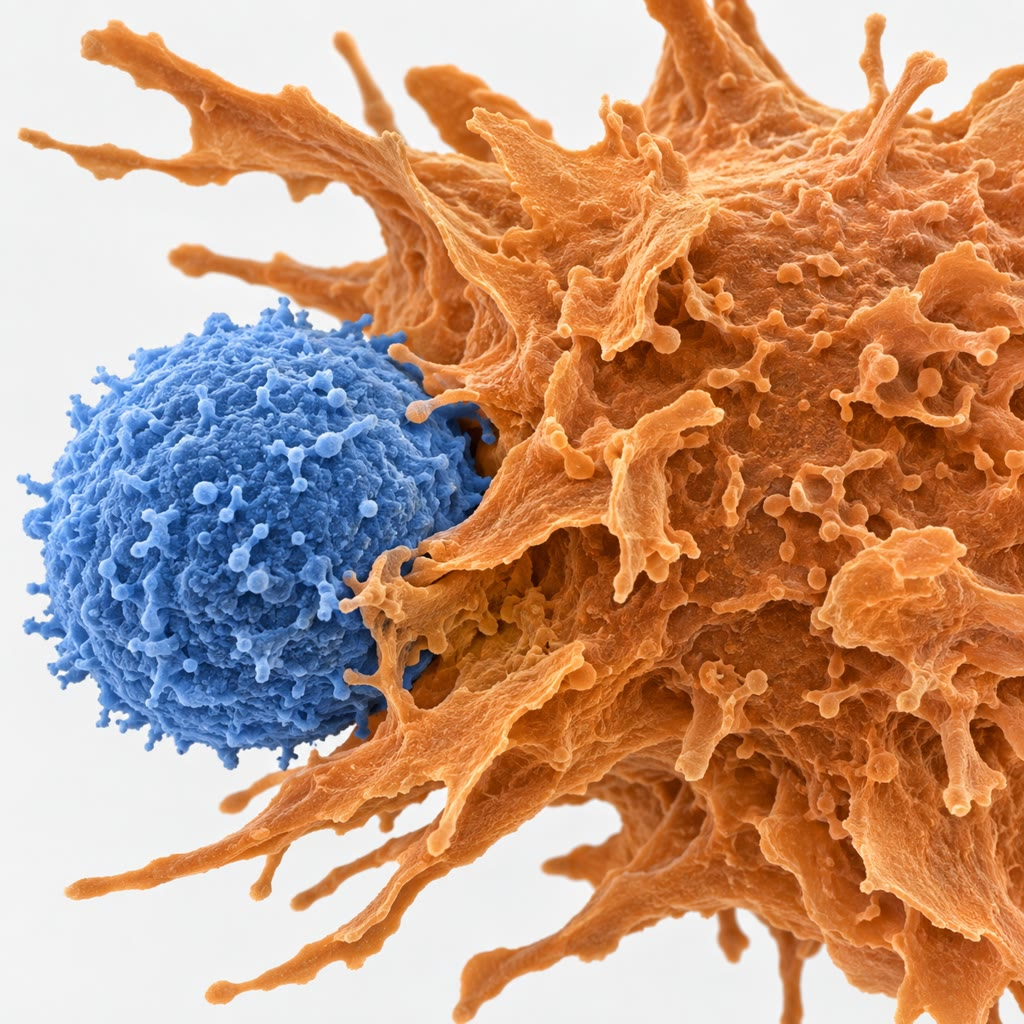
\includegraphics[width=0.36\linewidth]{images/book5/ai/b5-16-t-cell-apc.jpg}

{\small Kiri: sebuah \omterm{def:b3:adaptive-immunity:germinal-centre}{pusat germinal} di dalam sebuah \omterm{def:b3:adaptive-immunity:lymphocytes}{kelenjar limfa} --- zona
gelapnya yang padat dan zona seleksinya yang lebih terang. Kanan: sebuah sel~T
(kecil) yang bersentuhan dengan sebuah \omterm{def:b3:innate-immunity:innate}{sel dendritik}, yakni saat ketika
tanggapan adaptifnya diputuskan.}
\end{omfigure}

\section{Toleransi dan kegagalannya}

\begin{definition}[Toleransi]\label{def:b3:adaptive-immunity:tolerance}
\index{toleransi}\index{seleksi negatif}\index{timus}%
\index{anergi}\index{FoxP3}\index{autoimunitas}
Khazanahnya dibuat secara acak sehingga memuat reseptor bagi
diri. \emph{Toleransi pusat} menyingkirkannya di tempat selnya matang: di dalam
timusnya, sel~T yang reseptornya mengikat peptida--MHC diri terlalu kuat
dibunuh (\emph{seleksi negatif}), sel yang sama sekali tidak dapat mengikat MHC
juga dibunuh (sel itu akan tak berguna), dan hanya beberapa persen yang di
tengah yang pergi; sebuah faktor transkripsi, AIRE, membuat sel timusnya
mengungkapkan protein dari tiap jaringan --- insulin, tiroglobulin --- sehingga
sel~T yang khas baginya dapat dihapus di sana. Sel~B yang mengikat
diri di dalam sumsumnya dihapus atau menyunting reseptornya. \emph{Toleransi
tepi} menangani selebihnya: sebuah sel~T yang menjumpai \omterm{def:b3:adaptive-immunity:lymphocytes}{antigennya} tanpa
\omterm{def:b3:adaptive-immunity:response}{kostimulasi} dibuat tak tanggap (\emph{anergi}) atau dihapus; dan
sel~T \emph{pengatur}, yang didefinisikan faktor FoxP3, secara aktif
menekan tanggapan terhadap diri dan terhadap \omterm{def:b3:adaptive-immunity:lymphocytes}{antigen} tak berbahaya seperti
makanan dan komensal. \emph{Autoimunitas} adalah kegagalan kendali
ini: diabetes jenis~1 (sel~T memusnahkan sel $\beta$), sklerosis ganda
(mielin), radang sendi rematoid (sendi), dan lupus (yakni \omterm{def:b3:adaptive-immunity:antibody}{antibodi}
terhadap komponen inti), serta penyakit tiroid; masing-masing berkaitan dengan
alel \omterm{def:b3:adaptive-immunity:mhc}{HLA} tertentu, yang menyajikan peptida diri yang bersangkutan, dan
sebagian dipicu infeksi oleh sebuah mikroba yang peptidanya menyerupai
sebuah protein diri (demam rematik sesudah infeksi streptokokus).
\end{definition}

\begin{proof}[Bukti eksperimental]
Medawar (1953) menyuntikkan sel dari satu galur mencit kawin dalam ke dalam
mencit yang baru lahir dari galur lain; ketika dewasa, penerimanya menerima
cangkok kulit dari galur donornya yang jika tidak demikian akan ditolaknya,
sambil menolak cangkok dari galur ketiga. \omterm{def:b3:adaptive-immunity:tolerance}{Toleransinya} diperoleh, khas,
dan ditetapkan oleh apa yang dijumpai sistem imunnya sejak awal --- yakni dasar
percobaan bagi penghapusan klona reaktif diri milik Burnet. Anak yang lahir
tanpa gen AIRE yang berfungsi mengembangkan \omterm{def:b3:adaptive-immunity:tolerance}{autoimunitas} terhadap banyak organ
sekaligus; anak yang tanpa \omterm{def:b3:adaptive-immunity:tolerance}{FoxP3} (sebuah sindrom terkait-X yang langka)
mengembangkan \omterm{def:b3:adaptive-immunity:tolerance}{autoimunitas} yang mematikan pada masa bayi --- yakni kedua lengan
\omterm{def:b3:adaptive-immunity:tolerance}{toleransinya}, yang masing-masing ditunjukkan oleh ketiadaannya.
\end{proof}

\begin{example}[Hipersensitivitas, defisiensi, pencangkokan]\label{ex:b3:adaptive-immunity:failures}
\emph{Alergi} adalah sebuah tanggapan Th2 terhadap \omterm{def:b3:adaptive-immunity:lymphocytes}{antigen} tak berbahaya ---
serbuk sari, kacang tanah, penisilin --- yang menghasilkan IgE; pada pemaparan
ulang, \omterm{def:b3:adaptive-immunity:lymphocytes}{antigennya} menyilangkaitkan IgE pada sel mast, yang melepaskan histamin
dalam hitungan menit, dan bila \omterm{def:b3:adaptive-immunity:lymphocytes}{antigennya} ada di dalam darah, pelepasan
menyeluruhnya adalah \emph{anafilaksis}, yang diobati dengan adrenalin.
\emph{Imunodefisiensi}: anak yang tidak punya \omterm{def:b3:adaptive-immunity:antibody}{RAG} atau enzim ADA tidak membuat
\omterm{def:b3:adaptive-immunity:lymphocytes}{limfosit} (imunodefisiensi gabungan yang berat) lalu mati karena infeksi kecuali
diberi sumsum atau terapi gen; HIV memusnahkan sel~T CD4 dan bersamanya
pertolongan yang diperlukan tiap tanggapan. \emph{Pencangkokan}: sel~T
penerimanya melihat molekul \omterm{def:b3:adaptive-immunity:mhc}{HLA} donornya sebagai asing, dan sampai sepersepuluh
seluruh sel~T menanggapinya --- jauh lebih banyak daripada terhadap patogen mana
pun --- sehingga cangkoknya dicocokkan pada lokus \omterm{def:b3:adaptive-immunity:mhc}{HLA} dan penerimanya ditekan
imunitasnya seumur hidup; sebuah cangkok sumsum justru dapat menyerang inang
barunya. Lalu kegunaan yang disengaja: \omterm{def:b3:genetic-engineering:expression}{antibodi monoklonal}
\cref{ch:b3:genetic-engineering}, \omterm{prop:b3:cancer-biology:immune}{penghambat titik periksa} yang melepaskan
sel~T terhadap \omterm{def:b3:cancer-biology:hallmarks}{tumor} (\cref{ch:b3:cancer-biology}), serta sel~T yang direkayasa
dengan sebuah reseptor kimera bagi sebuah \omterm{def:b3:adaptive-immunity:lymphocytes}{antigen} \omterm{def:b3:cancer-biology:hallmarks}{tumor} (CAR-T), yang telah
menyembuhkan leukemia yang tidak tersentuh apa pun.
\end{example}

\section{Vaksinasi}

\begin{definition}[Vaksin dan imunitas kelompok]\label{def:b3:adaptive-immunity:vaccine}
\index{vaksin}\index{imunitas kelompok}%
\index{bilangan reproduksi dasar}\index{kemujaraban vaksin}
Sebuah \emph{vaksin} menyajikan \omterm{def:b3:adaptive-immunity:lymphocytes}{antigen} sebuah patogen, dengan sebuah ajuvan
atau dalam sebuah bentuk yang memicu reseptor bawaan, sehingga penerimanya
memperoleh \omterm{def:b3:adaptive-immunity:response}{sel ingatan} dan \omterm{def:b3:adaptive-immunity:antibody}{antibodi} tanpa penyakitnya
(\cref{ch:b3:virology} mendaftar jenisnya). \emph{Kemujaraban}-nya $E$ adalah
bagian orang tervaksinasi yang terlindungi. Perlindungannya meluas melampaui
yang tervaksinasi: sebuah patogen yang menyebar di dalam sebuah populasi yang
tiap kasusnya menginfeksi rata-rata $R_{0}$ orang lain ketika semuanya rentan
--- yakni \emph{bilangan reproduksi dasar} --- menginfeksi hanya $R_{0}$ kali
bagian yang rentan ketika sebagian sudah kebal, lalu lenyap ketika
bilangan itu jatuh di bawah satu. Inilah \emph{imunitas kelompok}: di atas sebuah
ambang orang yang kebal, rantai penularannya putus dan yang tidak tervaksinasi
--- bayi, orang yang lemah imunitasnya, orang yang vaksinnya gagal
--- terlindungi oleh yang lain.
\end{definition}

\begin{theorem}[Ambang imunitas kelompok]\label{thm:b3:adaptive-immunity:herd}
\index{imunitas kelompok!ambang}\index{model SIR}
Pada sebuah populasi yang bagian $p$-nya kebal dan selebihnya
rentan, tiap kasus menginfeksi rata-rata $R_{\text{eff}} = R_{0}(1 -
p)$ orang lain. Sebuah wabah tidak dapat mulai bila $R_{\text{eff}} < 1$, yakni
bila
\[
p > p_{c} = 1 - \frac{1}{R_{0}} .
\]
Dengan sebuah \omterm{def:b3:adaptive-immunity:vaccine}{vaksin} berkemujaraban $E$, cakupan yang diperlukan adalah $f_{c} = p_{c}/E$.
Bila sebuah wabah memang berjalan di dalam populasi yang rentan (\omterm{thm:b3:adaptive-immunity:herd}{model SIR},
dengan laju infeksi $\beta$ dan laju pemulihan $\gamma$, $R_{0} =
\beta/\gamma$), ia memuncak ketika bagian yang rentan telah turun ke
$1/R_{0}$, dan bagian yang tidak pernah terinfeksi, $s_{\infty}$, memenuhi
$\ln s_{\infty} = -R_{0}(1 - s_{\infty})$.
\end{theorem}
\begin{proof}
Tiap kasus membuat sentuhan yang akan menginfeksi $R_{0}$ orang bila semuanya
rentan; bagian $1 - p$ di antaranya memang rentan, sehingga $R_{\text{eff}} =
R_{0}(1-p)$, dan syarat $R_{\text{eff}} < 1$ memberi $p_{c}$; sebuah
\omterm{def:b3:adaptive-immunity:vaccine}{vaksin} yang melindungi bagian $E$ dari orang yang menerimanya membuat
bagian $Ef$ populasinya kebal, sehingga $Ef > p_{c}$. Pada \omterm{thm:b3:adaptive-immunity:herd}{model
SIR}, $\mathrm{d}s/\mathrm{d}t = -\beta si$ dan $\mathrm{d}i/\mathrm{d}t =
\beta si - \gamma i = \gamma i(R_{0}s - 1)$, sehingga $i$ tumbuh selama $s >
1/R_{0}$ lalu turun sesudahnya: puncaknya pada $s = 1/R_{0}$. Dengan membagi
kedua persamaannya, $\mathrm{d}i/\mathrm{d}s = -1 + 1/(R_{0}s)$, sehingga $i + s -
\ln s/R_{0}$ tetap; menilainya pada awalnya ($s = 1$, $i
\approx 0$) dan pada akhirnya ($i = 0$, $s = s_{\infty}$) memberi
$s_{\infty} - \ln s_{\infty}/R_{0} = 1$, yakni hubungan ukuran akhirnya.
\end{proof}

\begin{example}[Campak dan cacar]\label{ex:b3:adaptive-immunity:measles}
Campak punya $R_{0} \approx 15$: $p_{c} = 1 - 1/15 = 93\,\%$, dan dengan
sebuah \omterm{def:b3:adaptive-immunity:vaccine}{vaksin} berkemujaraban $97\,\%$ sesudah dua dosis, cakupan yang diperlukan
adalah $96\,\%$ --- itulah sebabnya campak kembali di mana pun vaksinasinya
merosot beberapa persen, dan sebabnya seorang anak yang tidak divaksinasi di
sebuah negeri yang tervaksinasi baik toh aman. Cacar punya $R_{0} \approx 5$--$7$,
sebuah ambang dekat $80$--$85\,\%$, tanpa wadah hewan, tanpa pengusung
tanpa gejala, dan sebuah \omterm{def:b3:adaptive-immunity:vaccine}{vaksin} yang bekerja dalam satu dosis: dapat dibasmi, dan
telah dibasmi. Polio hampir sampai ke sana. Influenza dan koronavirus,
yang \omterm{def:b3:adaptive-immunity:lymphocytes}{antigennya} menghanyut (\cref{ch:b3:virology}) dan imunitasnya memudar,
tidak. Di dalam sebuah populasi yang tidak tervaksinasi, sebuah wabah dengan
$R_{0} = 3$ menginfeksi, menurut hubungan ukuran akhirnya,
$1 - s_{\infty} = 94\,\%$ orang; dengan $R_{0} = 1.5$, $58\,\%$.
\end{example}

\begin{omfigure}
\begin{tikzpicture}
\begin{axis}[
  width=6.4cm, height=5.4cm,
  axis x line=bottom, axis y line=left,
  xmin=1, xmax=18, ymin=0, ymax=1,
  xlabel={$R_{0}$}, ylabel={ambang $p_{c}$},
  xlabel style={font=\small, at={(axis description cs:0.5,-0.12)}, anchor=north}, ylabel style={font=\small},
  tick label style={font=\scriptsize}, xtick={1,3,6,9,12,15,18}, ytick={0,0.5,0.8,0.93,1}, yticklabels={0,0.5,0.8,0.93,1},
  clip=false,
]
\addplot[very thick, omDef, domain=1:18, samples=80] {1-1/x};
\fill[omThm] (axis cs:15,0.933) circle (2pt); \node[font=\scriptsize, anchor=south east] at (axis cs:15,0.94) {campak};
\fill[omThm] (axis cs:6,0.833) circle (2pt); \node[font=\scriptsize, anchor=north west] at (axis cs:6.3,0.82) {cacar};
\fill[omThm] (axis cs:2.5,0.6) circle (2pt); \node[font=\scriptsize, anchor=north west] at (axis cs:2.6,0.58) {influenza 1918};
\end{axis}
\begin{axis}[
  at={(7.6cm,0)}, anchor=south west,
  width=6.4cm, height=5.4cm,
  axis x line=bottom, axis y line=left,
  xmin=0, xmax=60, ymin=0, ymax=0.35,
  xlabel={hari}, ylabel={bagian yang menularkan},
  xlabel style={font=\small, at={(axis description cs:0.5,-0.12)}, anchor=north}, ylabel style={font=\small},
  tick label style={font=\scriptsize}, xtick={0,20,40,60}, ytick={0,0.1,0.2,0.3},
  clip=false,
]
\addplot[very thick, omThm, smooth] coordinates {(0,0.001) (5,0.003) (10,0.012) (15,0.04) (20,0.12) (25,0.25) (28,0.30) (31,0.27) (35,0.18) (40,0.09) (45,0.04) (50,0.015) (55,0.006) (60,0.002)};
\addplot[very thick, omDef, smooth] coordinates {(0,0.001) (5,0.0015) (10,0.0025) (15,0.004) (20,0.006) (25,0.009) (30,0.012) (35,0.014) (40,0.015) (45,0.014) (50,0.012) (55,0.009) (60,0.007)};
\node[font=\scriptsize, omThm, anchor=west] at (axis cs:30,0.3) {tanpa imunitas, $R_{0} = 3$};
\node[font=\scriptsize, omDef, anchor=south west] at (axis cs:32,0.03) {\qty{60}{\%} tervaksinasi: $R_{\text{eff}} = 1.2$};
\end{axis}
\end{tikzpicture}

{\small Kiri: ambangnya $1 - 1/R_{0}$ --- makin menular penyakitnya,
makin dekat ke semua orang yang harus kebal. Kanan: sebuah wabah SIR
dengan $R_{0} = 3$ pada populasi naif dan pada populasi yang \qty{60}{\%}
kebal, yang tidak cukup untuk menghentikannya tetapi mendataran dan melambatkannya.}
\end{omfigure}

\begin{omfigure}
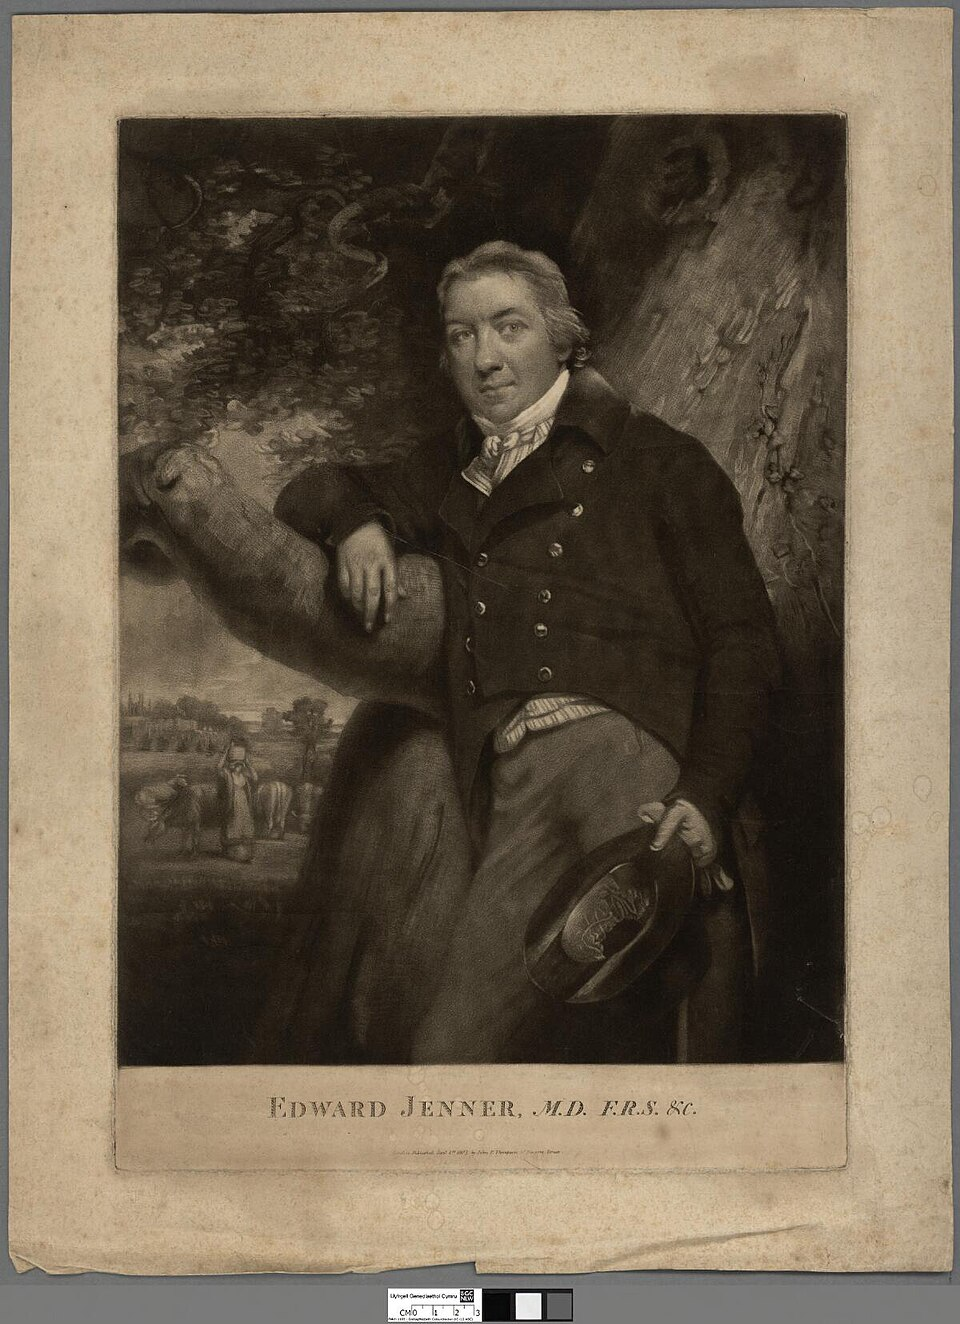
\includegraphics[width=0.30\linewidth]{images/book5/jenner.jpg}\hspace{0.04\linewidth}
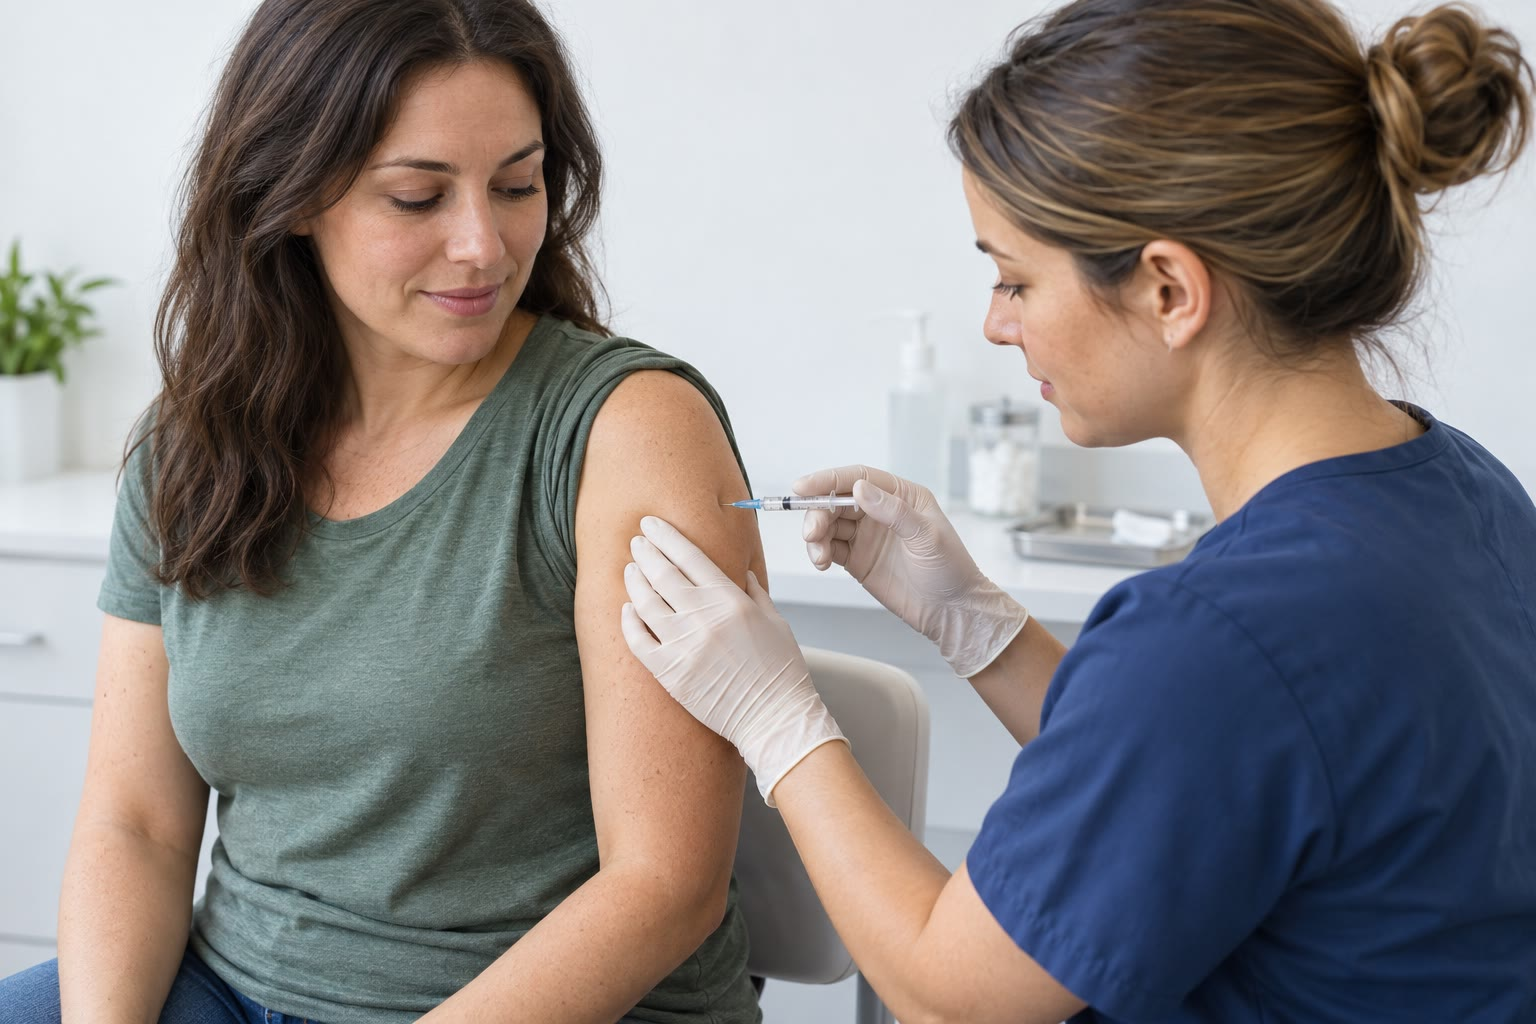
\includegraphics[width=0.50\linewidth]{images/book5/ai/b5-16-vaccination.jpg}

{\small Edward Jenner, yang pada tahun 1796 melindungi seorang anak lelaki dari
cacar dengan cacar sapi lalu mendirikan vaksinasi (ukiran tahun 1807, \omterm{def:b3:structural-biology:levels}{domain}
publik). Kanan: perbuatan yang sama dua abad kemudian --- sebuah \omterm{def:b3:adaptive-immunity:vaccine}{vaksin}
intramuskulus, yang \omterm{def:b3:adaptive-immunity:lymphocytes}{antigennya} akan diusung \omterm{def:b3:innate-immunity:innate}{sel dendritik} otot deltoid ke
\omterm{def:b3:adaptive-immunity:lymphocytes}{kelenjar limfa} ketiak.}
\end{omfigure}

\begin{remark}[Apa yang diingat imunitas]\label{rem:b3:adaptive-immunity:memory}
Sistem imun adaptif adalah sebuah mesin Darwin di dalam diri kita masing-masing:
ragam acak (V(D)J, hipermutasi), seleksi (oleh \omterm{def:b3:adaptive-immunity:lymphocytes}{antigen}, di dalam
\omterm{def:b3:adaptive-immunity:germinal-centre}{pusat germinal}, melawan diri di dalam \omterm{def:b3:adaptive-immunity:tolerance}{timus}), dan pewarisan (\omterm{def:b3:adaptive-immunity:response}{sel ingatan},
pengembangan klona). Ia menyelesaikan, dalam hitungan minggu, masalah yang
diselesaikan evolusi dalam ribuan tahun --- sebuah molekul yang mengikat sebuah
sasaran yang tak pernah dilihat sebelumnya --- dan jawabannya termasuk kasus
evolusi yang paling terpelajari yang teramati langsung. Ongkosnya adalah
\omterm{def:b3:adaptive-immunity:tolerance}{autoimunitas}, ketergantungannya pada pertimbangan sistem bawaannya mutlak, dan
ingatannya, yang dimanfaatkan Jenner dan yang ditulis \omterm{def:b3:adaptive-immunity:vaccine}{vaksin} dengan sengaja,
adalah alasan sebuah spesies hewan yang berumur panjang dan berbiak lambat dapat
bertahan hidup di dunia yang penuh mikroba yang berbiak cepat.
\end{remark}

\section{Latihan}

\begin{exercise}[$\star$]\label{exo:b3:adaptive-immunity:1}
Nyatakanlah keempat pokok \omterm{def:b3:adaptive-immunity:lymphocytes}{seleksi klonal} dan percobaan yang
mendukung masing-masing dari kedua yang pertama.
\end{exercise}

\begin{exercise}[$\star$]\label{exo:b3:adaptive-immunity:2}
Perikanlah struktur sebuah \omterm{def:b3:adaptive-immunity:antibody}{antibodi} lalu berilah fungsi tiap dari kelima
kelasnya.
\end{exercise}

\begin{exercise}[$\star$]\label{exo:b3:adaptive-immunity:3}
Pertentangkanlah \omterm{def:b3:adaptive-immunity:mhc}{MHC kelas~I} dan kelas~II pada sebaran selnya, sumber
peptidanya, panjang peptidanya, dan sel~T yang membaca masing-masing.
\end{exercise}

\begin{exercise}[$\star$]\label{exo:b3:adaptive-immunity:4}
Definisikanlah $R_{0}$ dan ambang \omterm{def:b3:adaptive-immunity:vaccine}{imunitas kelompok}, lalu hitunglah
ambangnya bagi gondongan ($R_{0} = 5$), batuk rejan ($R_{0} = 12$), dan
influenza 1918 ($R_{0} = 2.5$).
\end{exercise}

\begin{exercise}[$\star\star$]\label{exo:b3:adaptive-immunity:5}
Sebuah spesies punya $V_{H} = 50$, $D = 20$, $J_{H} = 5$ dan sebuah lokus
ringan tunggal dengan $V = 60$, $J = 4$. Hitunglah khazanah kombinatorisnya, lalu
totalnya dengan faktor sambungan $10^{4}$. Bagaimana perbandingannya
dengan $10^{9}$ sel~B yang dipunyai hewan itu?
\end{exercise}

\begin{exercise}[$\star\star$]\label{exo:b3:adaptive-immunity:6}
Daerah berubah-ubah sebuah sel~B \omterm{def:b3:adaptive-immunity:germinal-centre}{pusat germinal} sepanjang \qty{1000}{bp}; AID
memutasikannya pada $10^{-3}$ tiap pasangan basa tiap pembelahan. Sepanjang $20$
pembelahan, berapa banyak mutasi tiap sel, dan di antara $10^{5}$ sel berapa
banyak ragam basa tunggal \omterm{def:b3:adaptive-immunity:antibody}{antibodinya} yang dihasilkan? Bandingkanlah dengan
$3000$ substitusi tunggal yang mungkin.
\end{exercise}

\begin{exercise}[$\star\star$]\label{exo:b3:adaptive-immunity:7}
Jelaskanlah mengapa sebuah sel~T dari seseorang tidak mengenali peptida \omterm{def:b3:virology:virus}{virus}
yang disajikan sel orang lain, dan mengapa fakta yang sama itu membuat
pencangkokan sukar dan sistem \omterm{def:b3:adaptive-immunity:mhc}{HLA} polimorfik.
\end{exercise}

\begin{exercise}[$\star\star$]\label{exo:b3:adaptive-immunity:8}
Ramalkanlah fenotipe imun seorang anak yang tidak punya (a) RAG1, (b) AIRE,
(c) \omterm{def:b3:adaptive-immunity:tolerance}{FoxP3}, (d) enzim penukar kelas AID, dan (e) sel~T CD4.
\end{exercise}

\begin{exercise}[$\star\star$]\label{exo:b3:adaptive-immunity:9}
Sebuah \omterm{def:b3:adaptive-immunity:vaccine}{vaksin} berkemujaraban \qty{90}{\%} dan penyakitnya $R_{0} = 6$. Cakupan
berapa yang menghentikan penularannya? Bila cakupannya \qty{80}{\%}, berapa
$R_{\text{eff}}$-nya, dan berapa bagian populasi yang diinfeksi sebuah wabah
(pakailah hubungan ukuran akhirnya dengan $R_{0}$ diganti
$R_{\text{eff}}$ di antara yang rentan --- atau berhujahlah mengapa itu
kira-kira benar)?
\end{exercise}

\begin{exercise}[$\star\star\star$]\label{exo:b3:adaptive-immunity:10}
Turunkanlah hubungan ukuran akhir teoremanya dari persamaan SIR
lalu selesaikanlah secara numeris bagi $R_{0} = 1.5$, $2$, $3$, dan $5$. Mengapa
sebuah wabah tidak pernah menginfeksi semua orang bahkan tanpa campur tangan apa pun?
\end{exercise}

\begin{exercise}[$\star\star\star$]\label{exo:b3:adaptive-immunity:11}
\omterm{def:b3:adaptive-immunity:germinal-centre}{Pematangan afinitas} menaikkan pengikatannya seribu kali lipat dalam tiga minggu.
Perlakukanlah \omterm{def:b3:adaptive-immunity:germinal-centre}{pusat germinalnya} sebagai sebuah populasi di bawah seleksi: dengan
laju mutasi satu tiap sel tiap pembelahan, bagian $10^{-2}$ dari
mutasinya memperbaiki afinitas dengan faktor $1.5$ dan sisanya netral atau
merugikan, berapa putaran seleksi yang diperlukan bagi kenaikan seribu kali
lipat, dan berapa banyak sel yang harus disaring tiap putarannya? Berilah ulasan
mengapa \omterm{def:b3:adaptive-immunity:germinal-centre}{pusat germinalnya} ditata dalam daur.
\end{exercise}

\begin{exercise}[$\star\star\star$]\label{exo:b3:adaptive-immunity:12}
Penyakit autoimun lebih lazim pada perempuan dan berkaitan dengan alel
\omterm{def:b3:adaptive-immunity:mhc}{HLA}; diabetes jenis~1 telah naik lima kali lipat dalam lima puluh tahun di
negeri kaya. Usulkanlah, dengan mekanisme bab ini dan
\cref{ch:b3:microbiomes}, penjelasan bagi tiap pengamatan itu dan satu
ujinya masing-masing.
\end{exercise}

\section{Soal: Sebuah Kampanye Vaksin}

\begin{problem}[{Soal akhir pekan --- sebuah khazanah yang dicacah, sebuah
tanggapan yang ditakar waktunya dari seratus sel sampai semililiter serum, sebuah
pusat germinal yang dijalankan sebagai algoritme evolusi, serta sebuah kampanye
campak yang dirancang terhadap ambang kelompoknya, berakhir pada besar khazanahnya,
antibodi yang dibuat sebuah sel plasma sehari, dan cakupan yang diperlukan sebuah negeri}]
\label{pb:b3:adaptive-immunity:1}
Data: $V_{H} = 40$, $D = 25$, $J_{H} = 6$; lokus ringan $(40, 5)$ dan
$(30, 4)$; faktor sambungan $3\times 10^{4}$. Sebuah tubuh punya $10^{11}$
sel~B; satu dari $10^{5}$ mengikat sebuah epitop tertentu; $100$ pendahulu
direkrut; pembelahan tiap \qty{8}{h} selama $7$ hari; \qty{30}{\%} dari
klonanya menjadi \omterm{def:b3:adaptive-immunity:response}{sel plasma} yang menyekresikan $2000$ molekul IgG tiap detik
masing-masing; IgG sebesar \qty{150}{kDa}; volume plasma \qty{3}{L}; paruh hidup IgG
\qty{21}{d}. \omterm{def:b3:adaptive-immunity:germinal-centre}{Pusat germinal}: daerah berubah-ubah \qty{1000}{bp}, $10^{-3}$
mutasi tiap bp tiap pembelahan, satu dari $100$ mutasi memperbaiki
afinitas sebesar $1.5$. Campak: $R_{0} = 15$, \omterm{def:b3:adaptive-immunity:vaccine}{kemujaraban vaksin} $0.93$
sesudah satu dosis dan $0.97$ sesudah dua dosis; sebuah negeri berpenduduk $5\times 10^{6}$
orang dengan $60\,000$ kelahiran setahun.

\medskip
\noindent\textbf{Bagian I --- Khazanahnya.}
\begin{enumerate}
  \item Hitunglah khazanah kombinatorisnya dan totalnya dengan
        \omterm{def:b3:adaptive-immunity:antibody}{keanekaan sambungan}.
  \item Bandingkanlah dengan cacah sel~B. Berapa bagian khazanah yang
        mungkin yang diungkapkan satu tubuh pada satu saat, dan apa
        akibatnya bagi khazanah dua orang?
  \item Berapa banyak sel~B di dalam tubuhnya yang mengikat epitopnya? Berapa
        banyak, rata-rata, di dalam sebuah \omterm{def:b3:adaptive-immunity:lymphocytes}{kelenjar limfa} yang memuat $10^{8}$ sel~B?
  \item Seorang bayi baru lahir punya $10^{9}$ sel~B. Berapa banyak yang mengikat
        epitopnya, dan mengapa tanggapan bayi baru lahir toh lemah?
  \item Gelung ketiga rantai berat sebuah \omterm{def:b3:adaptive-immunity:antibody}{antibodi} dibuat oleh \omterm{def:b3:adaptive-immunity:antibody}{keanekaan
        sambungan}. Jelaskanlah mengapa gelung ini bagian yang paling
        berubah-ubah dari molekulnya dan biasanya di tengah tapak pengikatnya.
  \item \omterm{def:b3:adaptive-immunity:germinal-centre}{Hipermutasi somatik} menambahkan keanekaan sesudah seleksi, V(D)J
        sebelumnya. Mengapa menguntungkan punya keduanya, dalam urutan itu?
\end{enumerate}

\medskip
\noindent\textbf{Bagian II --- Tanggapannya.}
\begin{enumerate}[resume]
  \item Dari $100$ sel yang membelah tiap \qty{8}{h}, berapa banyak sesudah $7$
        hari? Berapa banyak \omterm{def:b3:adaptive-immunity:response}{sel plasma}?
  \item Berapa banyak molekul IgG yang disekresikannya tiap hari, dan berapa massanya?
        Kepekatan serum berapa yang diberikan keluaran sehari di dalam
        \qty{3}{L}?
  \item Sesudah sepuluh hari penyekresian pada laju itu, dengan mengabaikan
        peluruhannya, berapa kepekatannya dalam g/L? Bandingkanlah dengan IgG
        total yang normal sebesar \qty{10}{g/L}.
  \item \omterm{def:b3:adaptive-immunity:response}{Sel plasmanya} mati sesudah dua minggu; \omterm{def:b3:adaptive-immunity:antibody}{antibodinya} lalu meluruh
        dengan paruh hidup \qty{21}{d}. Berapa lama sampai kepekatan
        pertanyaan 9 turun seratus kali lipat? Apa yang mempertahankan \omterm{def:b3:adaptive-immunity:antibody}{antibodinya}
        bertahun-tahun?
  \item Sebuah tanggapan sekunder bermula dari $10^{5}$ \omterm{def:b3:adaptive-immunity:response}{sel ingatan}. Berapa
        banyak sel sesudah $3$ hari, dan bagaimana perbandingannya dengan
        tanggapan primer pada hari 3 dan hari 7?
  \item Jelaskanlah mengapa IgM datang lebih dulu dan IgG kemudian pada sebuah
        tanggapan primer, dan mengapa tanggapan sekundernya berupa IgG sejak awal.
\end{enumerate}

\medskip
\noindent\textbf{Bagian III --- \omterm{def:b3:adaptive-immunity:germinal-centre}{Pusat germinalnya}.}
\begin{enumerate}[resume]
  \item Berapa banyak mutasi yang diperoleh sebuah sel~B di daerah berubah-ubahnya
        tiap pembelahan? Sepanjang $20$ pembelahan?
  \item Berapa bagian anakan satu pembelahan yang mengusung sebuah
        mutasi yang memperbaiki? Di dalam sebuah \omterm{def:b3:adaptive-immunity:germinal-centre}{pusat germinal} berisi $10^{4}$ sel
        yang membelah, berapa banyak sel yang membaik muncul tiap pembelahan?
  \item Berapa banyak perbaikan berturut-turut sebesar $1.5$ yang memberi kenaikan
        afinitas seribu kali lipat? Bila tiap putaran seleksi memakan dua
        pembelahan (\qty{12}{h}), berapa lama itu?
  \item Kebanyakan mutasi merusak \omterm{def:b3:adaptive-immunity:antibody}{antibodinya}. Bila \qty{50}{\%} mutasinya
        memusnahkan pengikatannya, berapa bagian sel yang selamat dari mutasi tiap
        pembelahannya, dan mengapa zona terangnya harus membunuh kebanyakan selnya?
  \item Sebuah \omterm{def:b3:adaptive-immunity:vaccine}{vaksin} yang diberikan dalam dua dosis berjarak enam minggu menghasilkan
        \omterm{def:b3:adaptive-immunity:antibody}{antibodi} berafinitas lebih tinggi daripada satu dosis. Jelaskanlah dengan \omterm{def:b3:adaptive-immunity:germinal-centre}{pusat
        germinalnya}.
  \item Sebagian \omterm{def:b3:virology:virus}{virus} (HIV, influenza) lolos dari \omterm{def:b3:adaptive-immunity:antibody}{antibodi} dengan memutasikan
        permukaannya. Jelaskanlah mengapa \omterm{def:b3:adaptive-immunity:germinal-centre}{pusat germinalnya} toh
        menjadi dasar harapan bagi sebuah \omterm{def:b3:adaptive-immunity:vaccine}{vaksin} yang melindungi secara luas.
\end{enumerate}

\medskip
\noindent\textbf{Bagian IV --- Kampanyenya.}
\begin{enumerate}[resume]
  \item Ambang kelompok bagi campak, dan cakupan yang diperlukan dengan satu
        dosis; dengan dua dosis.
  \item Negeri itu memvaksinasi \qty{90}{\%} anak dengan dua dosis.
        Bagian yang kebal, $R_{\text{eff}}$, dan putusannya: apakah campak
        beredar?
  \item Berapa banyak anak rentan yang menimbun tiap tahun kelahiran pada
        cakupan \qty{90}{\%} (yang tidak tervaksinasi ditambah kegagalan \omterm{def:b3:adaptive-immunity:vaccine}{vaksin})? Sesudah
        lima tahun tanpa campak, berapa banyak orang rentannya,
        dan mengapa sebuah pemasukan lalu menyebabkan sebuah letusan?
  \item Pakailah hubungan ukuran akhirnya dengan bilangan reproduksi
        efektif di antara yang rentan untuk menaksir berapa bagian orang
        rentan itu yang diinfeksi sebuah letusan. (Ambillah $R_{\text{eff}}$ dari
        pertanyaan 20 sebagai bilangan reproduksi di seluruh populasinya,
        dan perhatikanlah bahwa di antara kumpulan yang rentan penyakitnya menyebar
        seolah-olah $R_{0}$ adalah $R_{\text{eff}}$.)
  \item Cakupannya dinaikkan ke \qty{95}{\%} dengan dua dosis. Bagian yang
        kebal dan $R_{\text{eff}}$; apakah ambangnya terpenuhi?
  \item Bayi di bawah setahun tidak dapat divaksinasi terhadap campak
        dan paling mungkin mati karenanya. Jelaskanlah bagaimana kampanyenya
        melindungi mereka, dan apa yang terjadi pada perlindungannya bila cakupannya
        turun ke \qty{85}{\%}.
  \item Ringkaslah: khazanah totalnya (pertanyaan~1), IgG yang dibuat \omterm{def:b3:adaptive-immunity:response}{sel
        plasma} sehari (pertanyaan~8), dan cakupan dua dosis yang
        diperlukan negeri itu (pertanyaan~19).
\end{enumerate}
\end{problem}
